% Options for packages loaded elsewhere
\PassOptionsToPackage{unicode}{hyperref}
\PassOptionsToPackage{hyphens}{url}
\documentclass[
  ignorenonframetext,
]{beamer}
\newif\ifbibliography
\usepackage{pgfpages}
\setbeamertemplate{caption}[numbered]
\setbeamertemplate{caption label separator}{: }
\setbeamercolor{caption name}{fg=normal text.fg}
\beamertemplatenavigationsymbolsempty
% remove section numbering
\setbeamertemplate{part page}{
  \centering
  \begin{beamercolorbox}[sep=16pt,center]{part title}
    \usebeamerfont{part title}\insertpart\par
  \end{beamercolorbox}
}
\setbeamertemplate{section page}{
  \centering
  \begin{beamercolorbox}[sep=12pt,center]{section title}
    \usebeamerfont{section title}\insertsection\par
  \end{beamercolorbox}
}
\setbeamertemplate{subsection page}{
  \centering
  \begin{beamercolorbox}[sep=8pt,center]{subsection title}
    \usebeamerfont{subsection title}\insertsubsection\par
  \end{beamercolorbox}
}
% Prevent slide breaks in the middle of a paragraph
\widowpenalties 1 10000
\raggedbottom
\AtBeginPart{
  \frame{\partpage}
}
\AtBeginSection{
  \ifbibliography
  \else
    \frame{\sectionpage}
  \fi
}
\AtBeginSubsection{
  \frame{\subsectionpage}
}
\usepackage{iftex}
\ifPDFTeX
  \usepackage[T1]{fontenc}
  \usepackage[utf8]{inputenc}
  \usepackage{textcomp} % provide euro and other symbols
\else % if luatex or xetex
  \usepackage{unicode-math} % this also loads fontspec
  \defaultfontfeatures{Scale=MatchLowercase}
  \defaultfontfeatures[\rmfamily]{Ligatures=TeX,Scale=1}
\fi
\usepackage{lmodern}
\ifPDFTeX\else
  % xetex/luatex font selection
\fi
% Use upquote if available, for straight quotes in verbatim environments
\IfFileExists{upquote.sty}{\usepackage{upquote}}{}
\IfFileExists{microtype.sty}{% use microtype if available
  \usepackage[]{microtype}
  \UseMicrotypeSet[protrusion]{basicmath} % disable protrusion for tt fonts
}{}
\makeatletter
\@ifundefined{KOMAClassName}{% if non-KOMA class
  \IfFileExists{parskip.sty}{%
    \usepackage{parskip}
  }{% else
    \setlength{\parindent}{0pt}
    \setlength{\parskip}{6pt plus 2pt minus 1pt}}
}{% if KOMA class
  \KOMAoptions{parskip=half}}
\makeatother
\usepackage{longtable,booktabs,array}
\usepackage{caption}
\captionsetup[table]{skip=6pt}
\newcounter{none} % for unnumbered tables
\usepackage{calc} % for calculating minipage widths
\usepackage{caption}
% Make caption package work with longtable
\makeatletter
\def\fnum@table{\tablename~\thetable}
\makeatother
\usepackage{graphicx}
\makeatletter
\newsavebox\pandoc@box
\newcommand*\pandocbounded[1]{% scales image to fit in text height/width
  \sbox\pandoc@box{#1}%
  \Gscale@div\@tempa{\textheight}{\dimexpr\ht\pandoc@box+\dp\pandoc@box\relax}%
  \Gscale@div\@tempb{\linewidth}{\wd\pandoc@box}%
  \ifdim\@tempb\p@<\@tempa\p@\let\@tempa\@tempb\fi% select the smaller of both
  \ifdim\@tempa\p@<\p@\scalebox{\@tempa}{\usebox\pandoc@box}%
  \else\usebox{\pandoc@box}%
  \fi%
}
% Set default figure placement to htbp
\def\fps@figure{htbp}
\makeatother
\setlength{\emergencystretch}{3em} % prevent overfull lines
\providecommand{\tightlist}{%
  \setlength{\itemsep}{0pt}\setlength{\parskip}{0pt}}
% Auto-generated by infrastructure/rendering/_pdf_latex_helpers.py::extract_math_font_preamble.
% Minimal header passed to Pandoc via -H so Beamer slides pick up the same math font
% as the combined-PDF path. Adjust the manuscript's preamble.md to change the font globally.
\usepackage{unicode-math}
\setmathfont{latinmodern-math.otf}

% Slide layout defaults for warning-clean scientific decks.
\usepackage{etoolbox}
\IfFileExists{xurl.sty}{\usepackage{xurl}}{}
\IfFileExists{seqsplit.sty}{\usepackage{seqsplit}}{\newcommand{\seqsplit}[1]{#1}}
\protected\def\breakseq#1{\seqsplit{#1}}
\protected\def\breaktt#1{\begingroup\ttfamily\seqsplit{#1}\endgroup}
\setlength{\emergencystretch}{6em}
\tolerance=5000
\hbadness=10000
\hfuzz=1pt
\setlength{\tabcolsep}{2pt}
\AtBeginEnvironment{longtable}{\tiny\renewcommand{\arraystretch}{0.86}\setlength{\tabcolsep}{1pt}}
\AtBeginEnvironment{tabular}{\tiny\renewcommand{\arraystretch}{0.86}\setlength{\tabcolsep}{1pt}}
\AtBeginEnvironment{equation}{\tiny}
\AtBeginEnvironment{equation*}{\tiny}
\AtBeginEnvironment{align}{\tiny}
\AtBeginEnvironment{align*}{\tiny}
\AtBeginEnvironment{itemize}{\footnotesize}
\AtBeginEnvironment{enumerate}{\footnotesize}
\AtBeginEnvironment{description}{\footnotesize}
\setbeamerfont{caption}{size=\tiny}
\setbeamerfont{caption name}{size=\tiny}
\setbeamerfont{normal text}{size=\small}
\setbeamerfont{frametitle}{size=\small}
\setbeamerfont{section title}{size=\footnotesize}
\setbeamerfont{subsection title}{size=\footnotesize}
\setbeamertemplate{section page}{%
  \centering
  \begin{beamercolorbox}[sep=12pt,center,wd=\paperwidth]{section title}
    \parbox{0.86\paperwidth}{\centering\usebeamerfont{section title}\insertsection\par}
  \end{beamercolorbox}
}
\setbeamertemplate{subsection page}{%
  \centering
  \begin{beamercolorbox}[sep=8pt,center,wd=\paperwidth]{subsection title}
    \parbox{0.86\paperwidth}{\centering\usebeamerfont{subsection title}\insertsubsection\par}
  \end{beamercolorbox}
}
\setlength{\abovecaptionskip}{2pt}
\setlength{\belowcaptionskip}{0pt}

% Natbib and cross-reference fallbacks — slides don't load natbib
% or cleveref, but combined-PDF manuscript prose may emit these
% commands. The fallback renders citations as a bracketed key list
% and cross-references as detokenized labels so slides don't fail on
% undefined control sequences or raw underscores. \providecommand is
% a no-op if packages load later.
\providecommand{\citep}[1]{[#1]}
\providecommand{\citet}[1]{#1}
\providecommand{\citealp}[1]{#1}
\providecommand{\citeauthor}[1]{#1}
\providecommand{\citeyear}[1]{#1}
\providecommand{\cref}[1]{\texttt{\detokenize{#1}}}
\providecommand{\Cref}[1]{\texttt{\detokenize{#1}}}

\newtheorem{proposition}{Proposition}
\newtheorem{hypothesis}{Hypothesis}
\usepackage{bookmark}
\IfFileExists{xurl.sty}{\usepackage{xurl}}{} % add URL line breaks if available
\urlstyle{same}
% fallback for those not using the hyperref driver hyperxmp:
\makeatletter
\@ifundefined{xmpquote}{\newcommand{\xmpquote}[1]{#1}}{}
\makeatother
\hypersetup{
  hidelinks,
  pdfcreator={LaTeX via pandoc}}

\author{\texorpdfstring{}{}}
\date{}

\begin{document}

\section{Results: Curriculum Graph and Assessment
Audits}\label{sec:results-curriculum-graph-assessment}

\begin{frame}[allowframebreaks]{Graph validity, prerequisite depth, and
assessment-quality gates}
\protect\phantomsection\label{graph-validity-prerequisite-depth-and-assessment-quality-gates}
The assembled curriculum is a valid directed acyclic graph of
\textbf{630 skills} in \textbf{111 subjects} joined by \textbf{1199
prerequisite edges}, spanning all 8 strata with a maximum prerequisite
depth of 75 and two foundational roots (set theory and the probability
axioms). Validation passes: no cycles, no dangling prerequisites, and
every applications skill is reachable from a foundational root.
fig.~\ref{fig:curriculum_dag} lays the graph out by stratum and depth,
uses wrapped stratum-count labels and root annotations, and reports the
maximum-depth summary.

\end{frame}

\begin{frame}[allowframebreaks]{Graph validity, prerequisite depth, and
assessment-quality gates}
The learner-quality gate then checks whether that valid graph is also
usable as a micro-learning catalog. Each skill has at least 4 failable
assessment items including a transfer-oriented multiple-choice check.
Answer position and answer length are then audited per answer-count
bucket, in every bucket carrying enough single-choice items to read.
Each option slot has to be correct at a rate inside a band around
chance, between \(0.10\) and \(0.45\) of the bucket, so no slot either
dominates or sits unused. The length check is two-sided: the rate at
which the correct option is the strictly longest answer and the rate at
which it is the strictly shortest answer must both land between \(0.12\)
and \(0.42\) of the bucket. Bounding only the long end would relocate
the cue rather than remove it, because an answer that is never the
longest teaches a learner to pick the shortest one. Multiple-choice
\end{frame}

\begin{frame}[allowframebreaks]{Graph validity, prerequisite depth, and
assessment-quality gates}
correctness is kept from collapsing onto a template: no option index
sits in the correct set for more than \(0.60\) of multiple-choice items,
and no single correct subset covers more than \(0.30\) of them.
Objective strings may repeat, but only within a bound --- at most four
skills may share one objective before the gate reports templated filler.
No single name-normalized answer body is reused across more than
\(0.12\) of skills, with the declared shared rubric exempted as
described below. Skill tags include both stratum and topic context, and
backward cross-stratum references are kept out of the exported
prerequisite path.

\end{frame}

\begin{frame}[allowframebreaks]{Graph validity, prerequisite depth, and
assessment-quality gates}
The one deliberately shared instrument is disclosed rather than hidden.
Each skill carries bespoke domain assessment items; most skills
additionally carry a shared transfer-and-misuse rubric, a uniform
metacognitive instrument applied across the curriculum and marked as
such. The answer-reuse gate exempts that declared rubric, requires every
skill to retain at least one bespoke item, and bounds every other
name-normalized answer body to at most \(0.12\) of skills. The exemption
is what makes that bound readable rather than misleading: each
per-family review rubric spans a whole stratum-by-role family, a
footprint above a tenth of the curriculum and therefore above the bound
the gate enforces on authored answers. We name the instrument and the
exemption instead of letting a shared rubric sit quietly under a
threshold, and the bespoke-item requirement keeps the rubric scaffolding
rather than a substitute for per-skill assessment.
\end{frame}

\begin{frame}[allowframebreaks]{Graph validity, prerequisite depth, and
assessment-quality gates}

These checks establish structural assessment discipline, not
psychometric validity. They show that quiz-gated completion is not thin,
duplicated, or position-biased under the local validators; they do not
estimate item reliability, construct validity, learner ability,
retention, transfer, or differential item functioning.

The headline depth of 75 is not a single conceptual chain. It is
dominated by the per-stratum mastery and open-science review ladders,
which sequence skills for completeness rather than by genuine conceptual
prerequisite. Excluding only those review and meta scaffold families and
keeping every genuine concept family (mathematics through applications,
plus the dynamical, geometric, hierarchical, implementation and
cognitive-security families), the substantive concept chain a learner
must climb is 33 deep; the difference is review and mastery sequencing,
not conceptual dependency. We report both so the headline number is not
\end{frame}

\begin{frame}[allowframebreaks]{Graph validity, prerequisite depth, and
assessment-quality gates}
read as the depth of the conceptual curriculum.

\end{frame}

\begin{frame}[allowframebreaks]{Graph validity, prerequisite depth, and
assessment-quality gates}
\begin{figure}
\centering
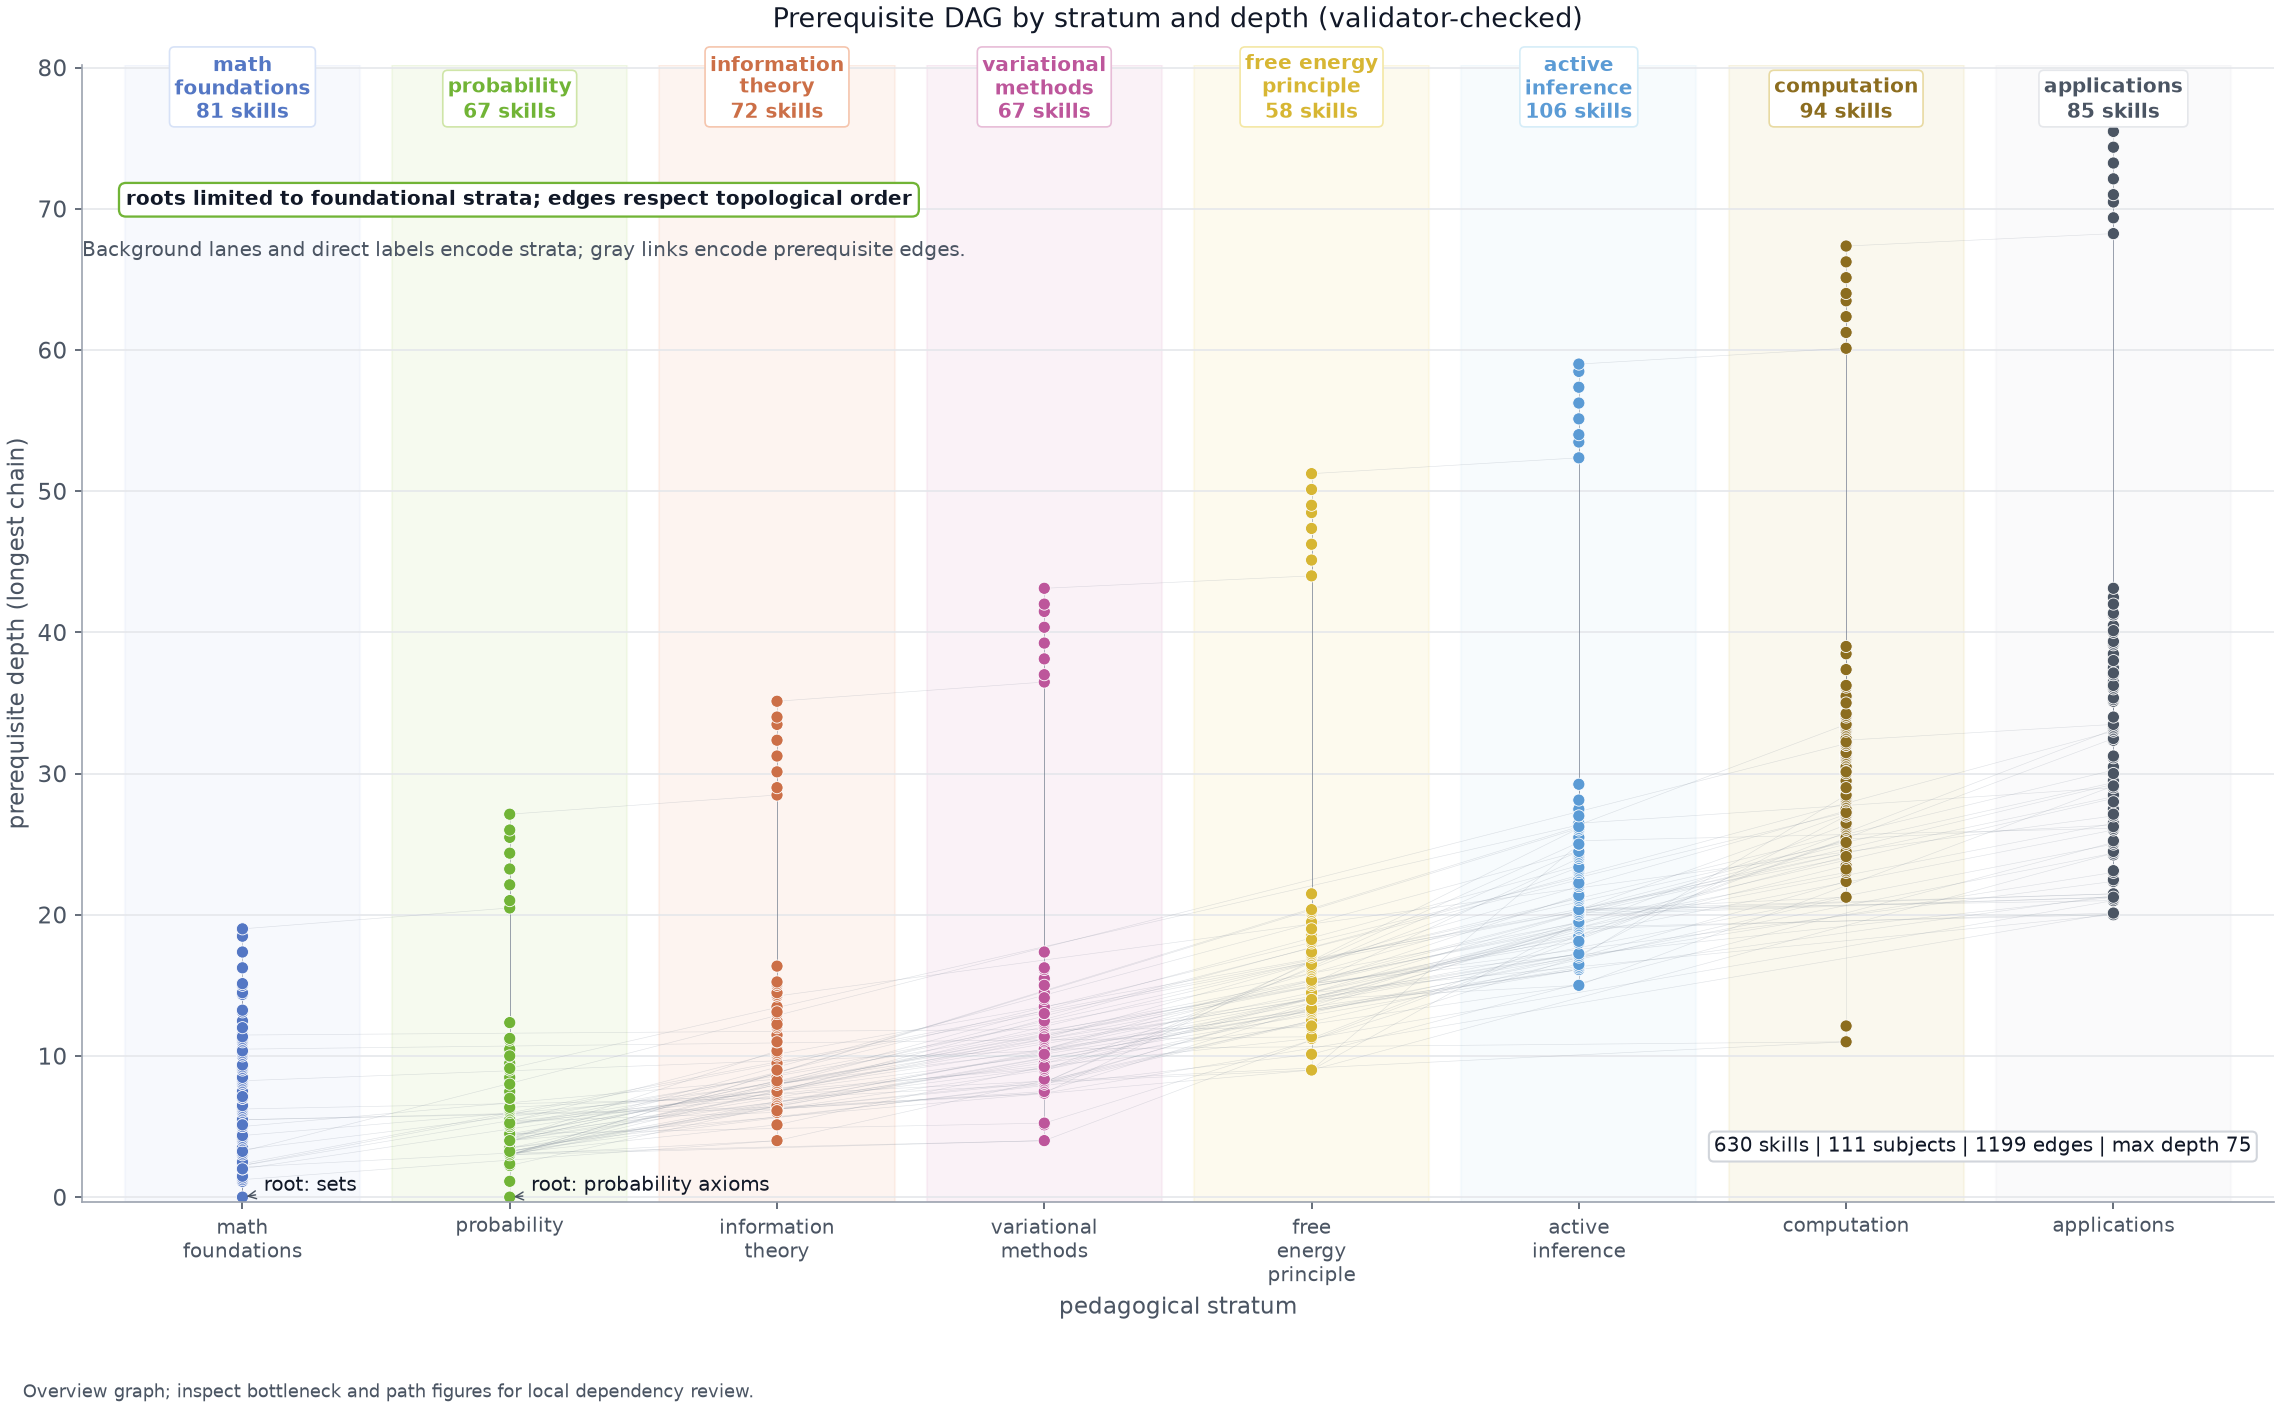
\includegraphics[width=1\linewidth,height=0.40\textheight,keepaspectratio,alt={The Active Inference curriculum as a prerequisite DAG generated from the current curriculum graph after structural checks. Each point is one skill, color encodes the pedagogical stratum, horizontal position follows the stratum order, vertical position follows longest prerequisite depth, and gray segments encode exported learning-path dependencies. Wrapped stratum chips report live skill totals, the two foundational roots are labeled, and the inset reports the live skill, subject, edge, and maximum-depth counts. This figure is an overview for structure and reachability; it does not by itself certify prose quality, assessment quality, or scholarship support.}]{../figures/curriculum_dag.png}
\caption{The Active Inference curriculum as a prerequisite DAG generated
from the current curriculum graph after structural checks. Each point is
one skill, color encodes the pedagogical stratum, horizontal position
follows the stratum order, vertical position follows longest
prerequisite depth, and gray segments encode exported learning-path
dependencies. Wrapped stratum chips report live skill totals, the two
foundational roots are labeled, and the inset reports the live skill,
subject, edge, and maximum-depth counts. This figure is an overview for
structure and reachability; it does not by itself certify prose quality,
assessment quality, or scholarship support.}\label{fig:curriculum_dag}
\end{figure}

\end{frame}

\begin{frame}[allowframebreaks]{Graph validity, prerequisite depth, and
assessment-quality gates}
The full DAG is the most faithful view, but it is intentionally dense:
learners need to see both the individual prerequisite chains and the
curriculum's aggregate traffic pattern.
fig.~\ref{fig:dependency_strata_flow} adds that second view. Rows are
prerequisite strata, columns are dependent strata, and the right-hand
bar gives the node count in each stratum. Diagonal cells show
within-stratum reinforcement; upper-triangular cells show forward
conceptual transitions. A populated lower-triangular cell would mean a
backward learning-path dependency, which the quality gate rejects before
export.

\end{frame}

\begin{frame}[allowframebreaks]{Graph validity, prerequisite depth, and
assessment-quality gates}
\begin{figure}
\centering
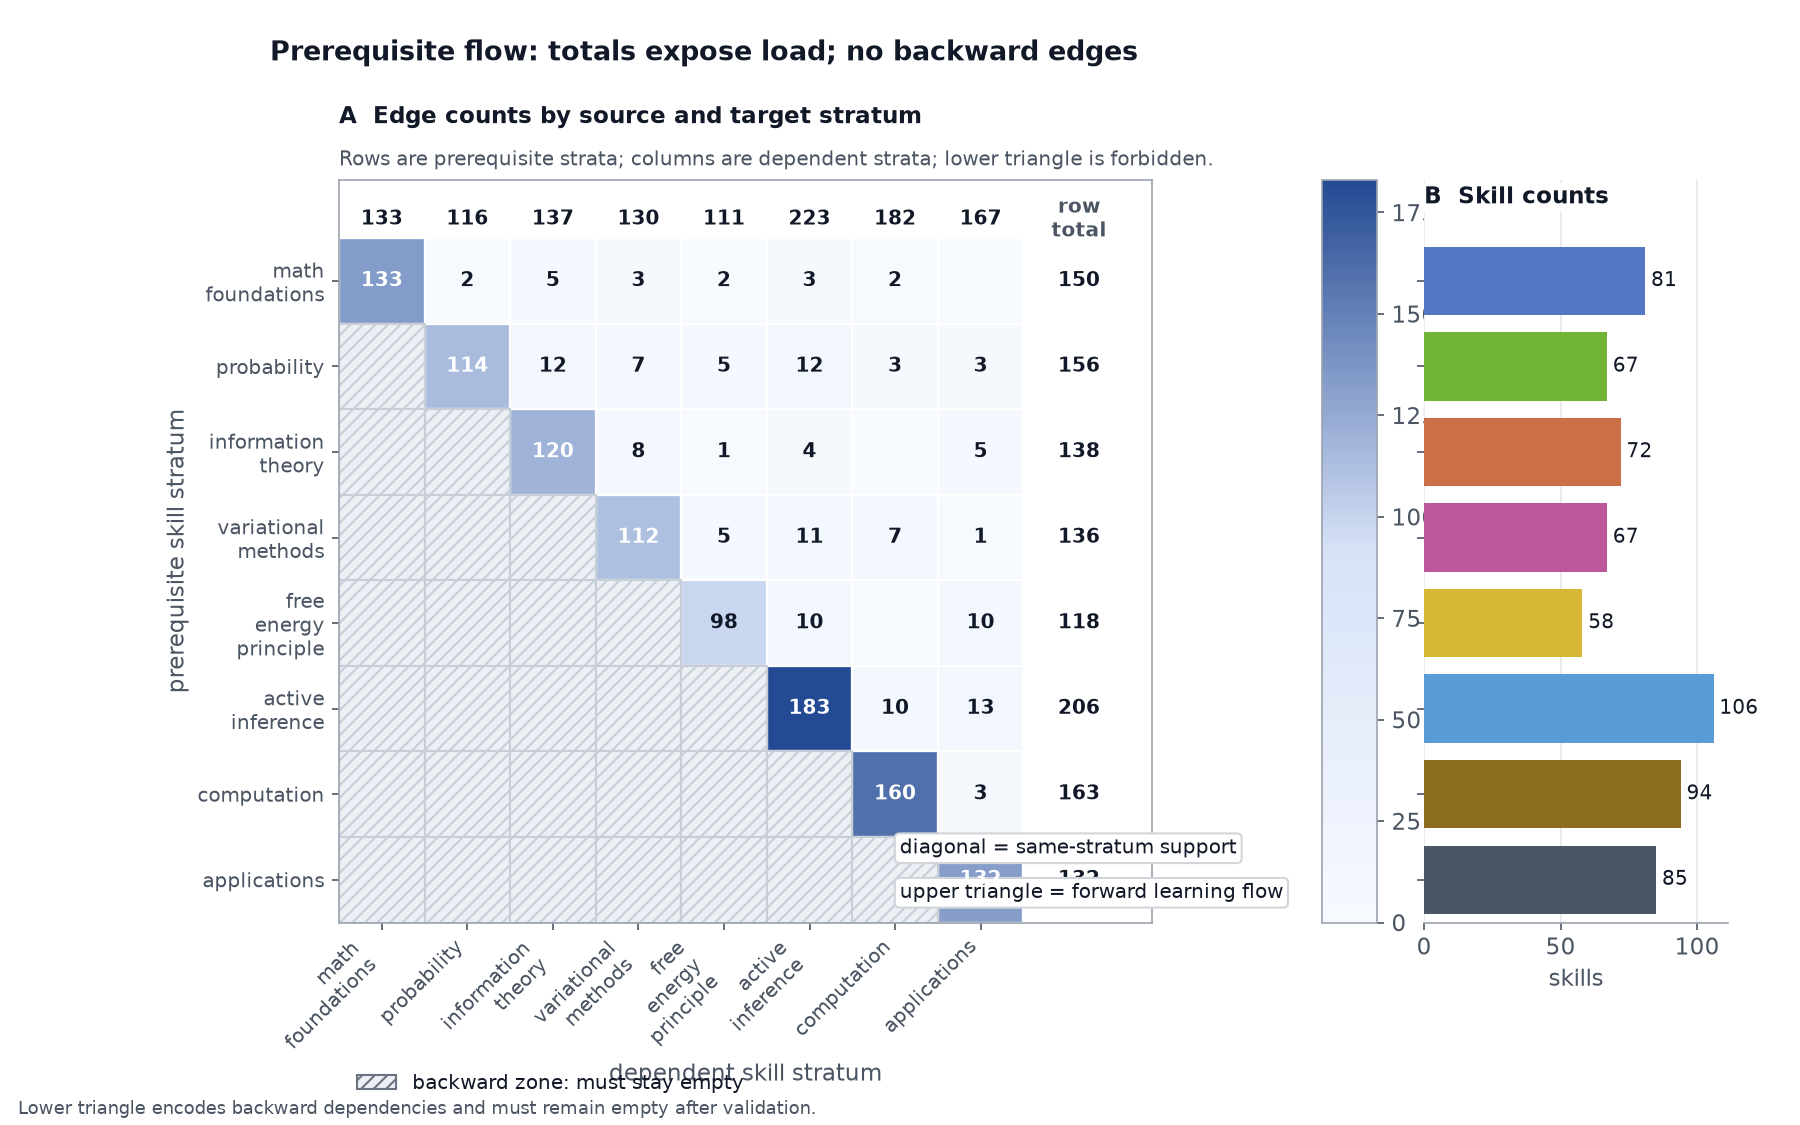
\includegraphics[width=0.95\linewidth,height=0.40\textheight,keepaspectratio,alt={Prerequisite-edge flow across strata generated from every exported learning-path edge. Rows are prerequisite strata, columns are dependent strata, cell labels count edges, and the side bar reports how many skills live in each stratum. Diagonal cells show within-stratum reinforcement, upper-triangular cells show forward conceptual transitions, and a populated lower-triangular cell would expose a backward prerequisite that should be rejected before export.}]{../figures/dependency_strata_flow.png}
\caption{Prerequisite-edge flow across strata generated from every
exported learning-path edge. Rows are prerequisite strata, columns are
dependent strata, cell labels count edges, and the side bar reports how
many skills live in each stratum. Diagonal cells show within-stratum
reinforcement, upper-triangular cells show forward conceptual
transitions, and a populated lower-triangular cell would expose a
backward prerequisite that should be rejected before
export.}\label{fig:dependency_strata_flow}
\end{figure}

\end{frame}

\begin{frame}[allowframebreaks]{Graph validity, prerequisite depth, and
assessment-quality gates}
The same graph also needs diagnostic views for authors.
fig.~\ref{fig:graph_bottlenecks} orders high-outdegree skills by how
much downstream curriculum they unlock, so review can focus on nodes
where a weak explanation would create wide learner risk.
fig.~\ref{fig:skill_neighborhood_paths} complements that global view
with a representative long dependency path. The figure keeps the route
line readable while a checkpoint ledger names the start, stratum
transitions, and endpoint, so a reader can inspect one concrete route
without zooming the full DAG or relying on angled micro-labels.

\end{frame}

\begin{frame}[allowframebreaks]{Graph validity, prerequisite depth, and
assessment-quality gates}
\begin{figure}
\centering
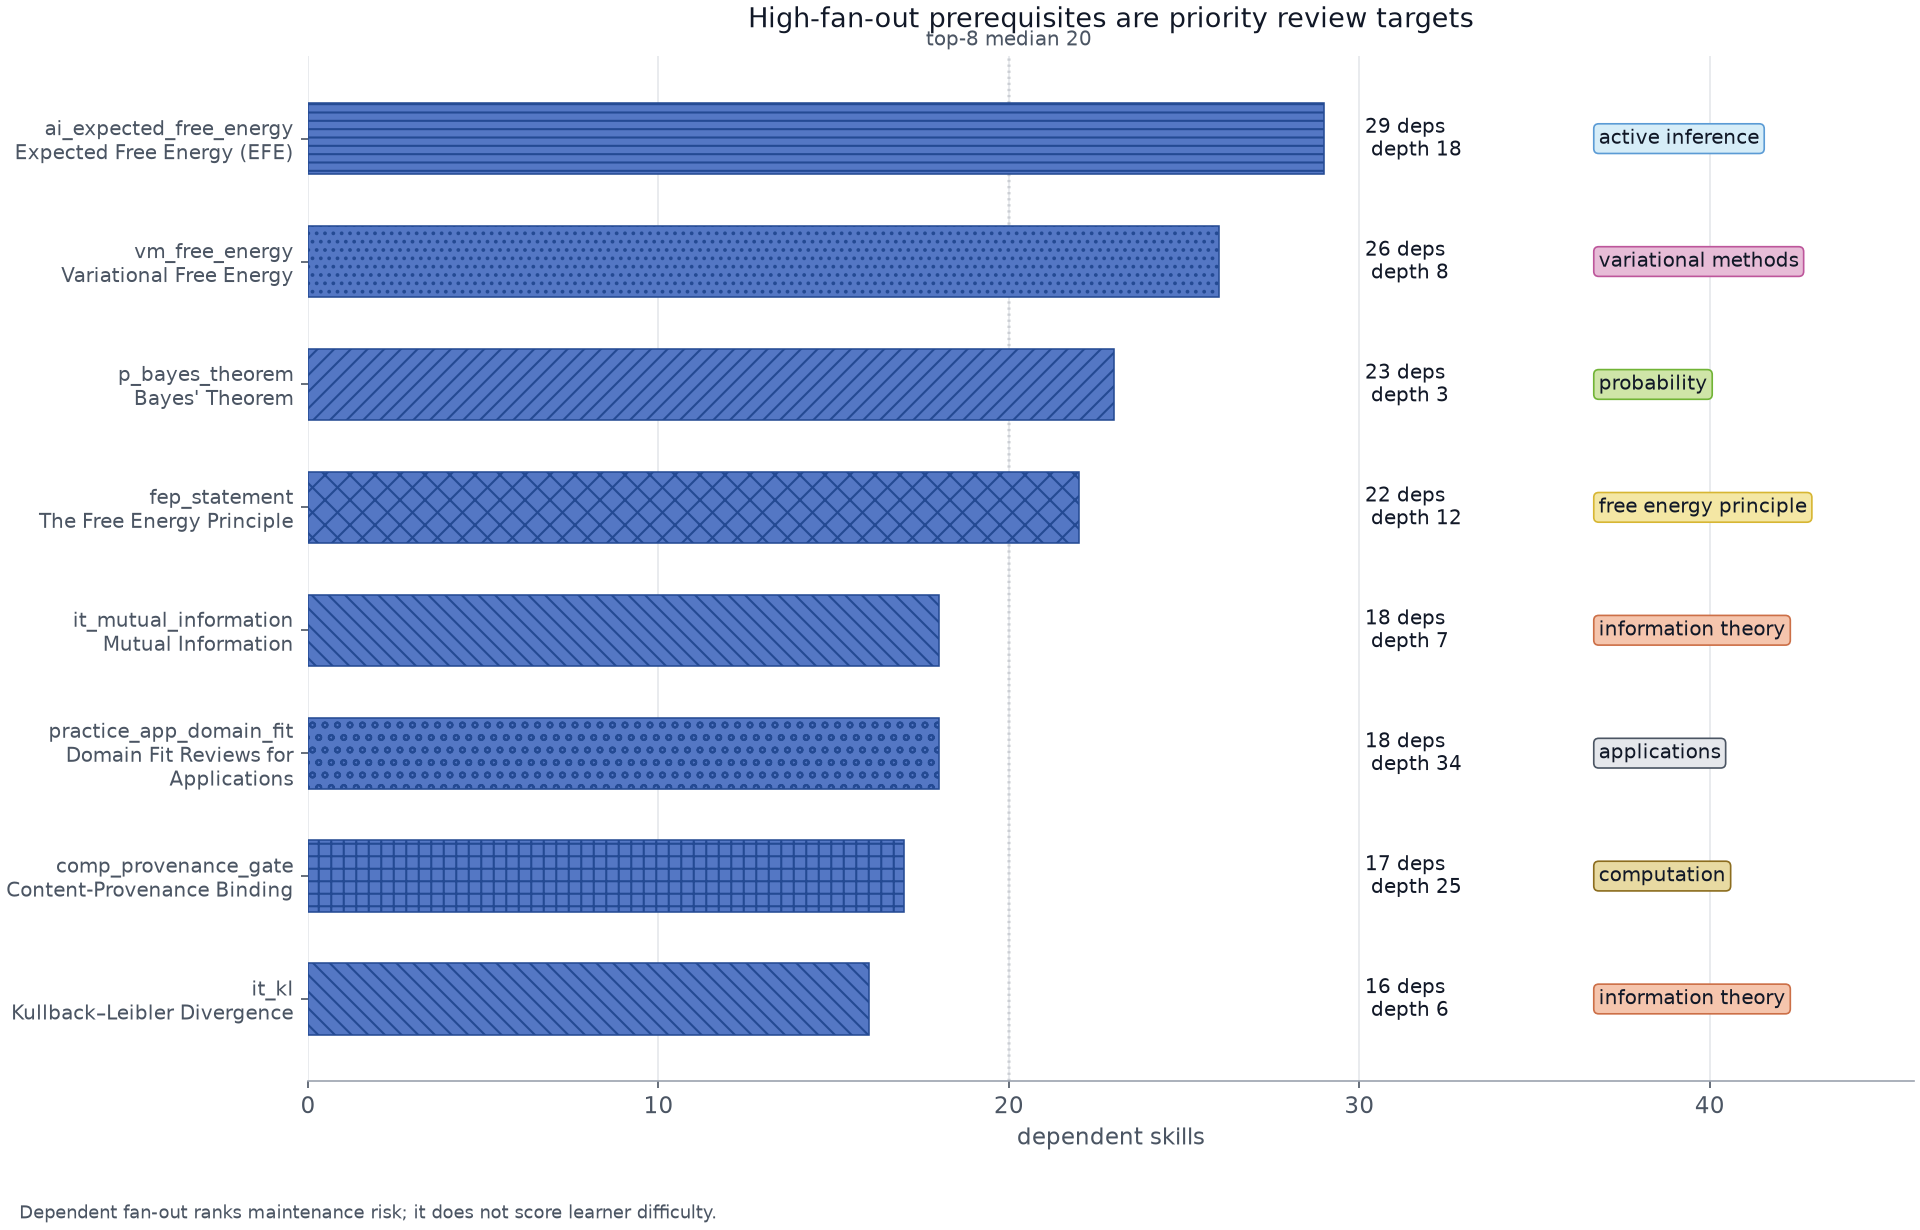
\includegraphics[width=0.92\linewidth,height=0.40\textheight,keepaspectratio,alt={Graph bottlenecks in the exported prerequisite network generated from downstream dependent counts. Bars rank the top fan-out skills, y-axis labels pair skill ids with readable names, hatching and stratum chips identify pedagogical layer, and annotations report dependent count and prerequisite depth for each high-impact node. The figure is a review-priority surface: it identifies where a weak explanation, stale citation, or thin quiz would propagate to many later skills even though the graph remains valid.}]{../figures/graph_bottlenecks.png}
\caption{Graph bottlenecks in the exported prerequisite network
generated from downstream dependent counts. Bars rank the top fan-out
skills, y-axis labels pair skill ids with readable names, hatching and
stratum chips identify pedagogical layer, and annotations report
dependent count and prerequisite depth for each high-impact node. The
figure is a review-priority surface: it identifies where a weak
explanation, stale citation, or thin quiz would propagate to many later
skills even though the graph remains
valid.}\label{fig:graph_bottlenecks}
\end{figure}

\begin{figure}
\centering
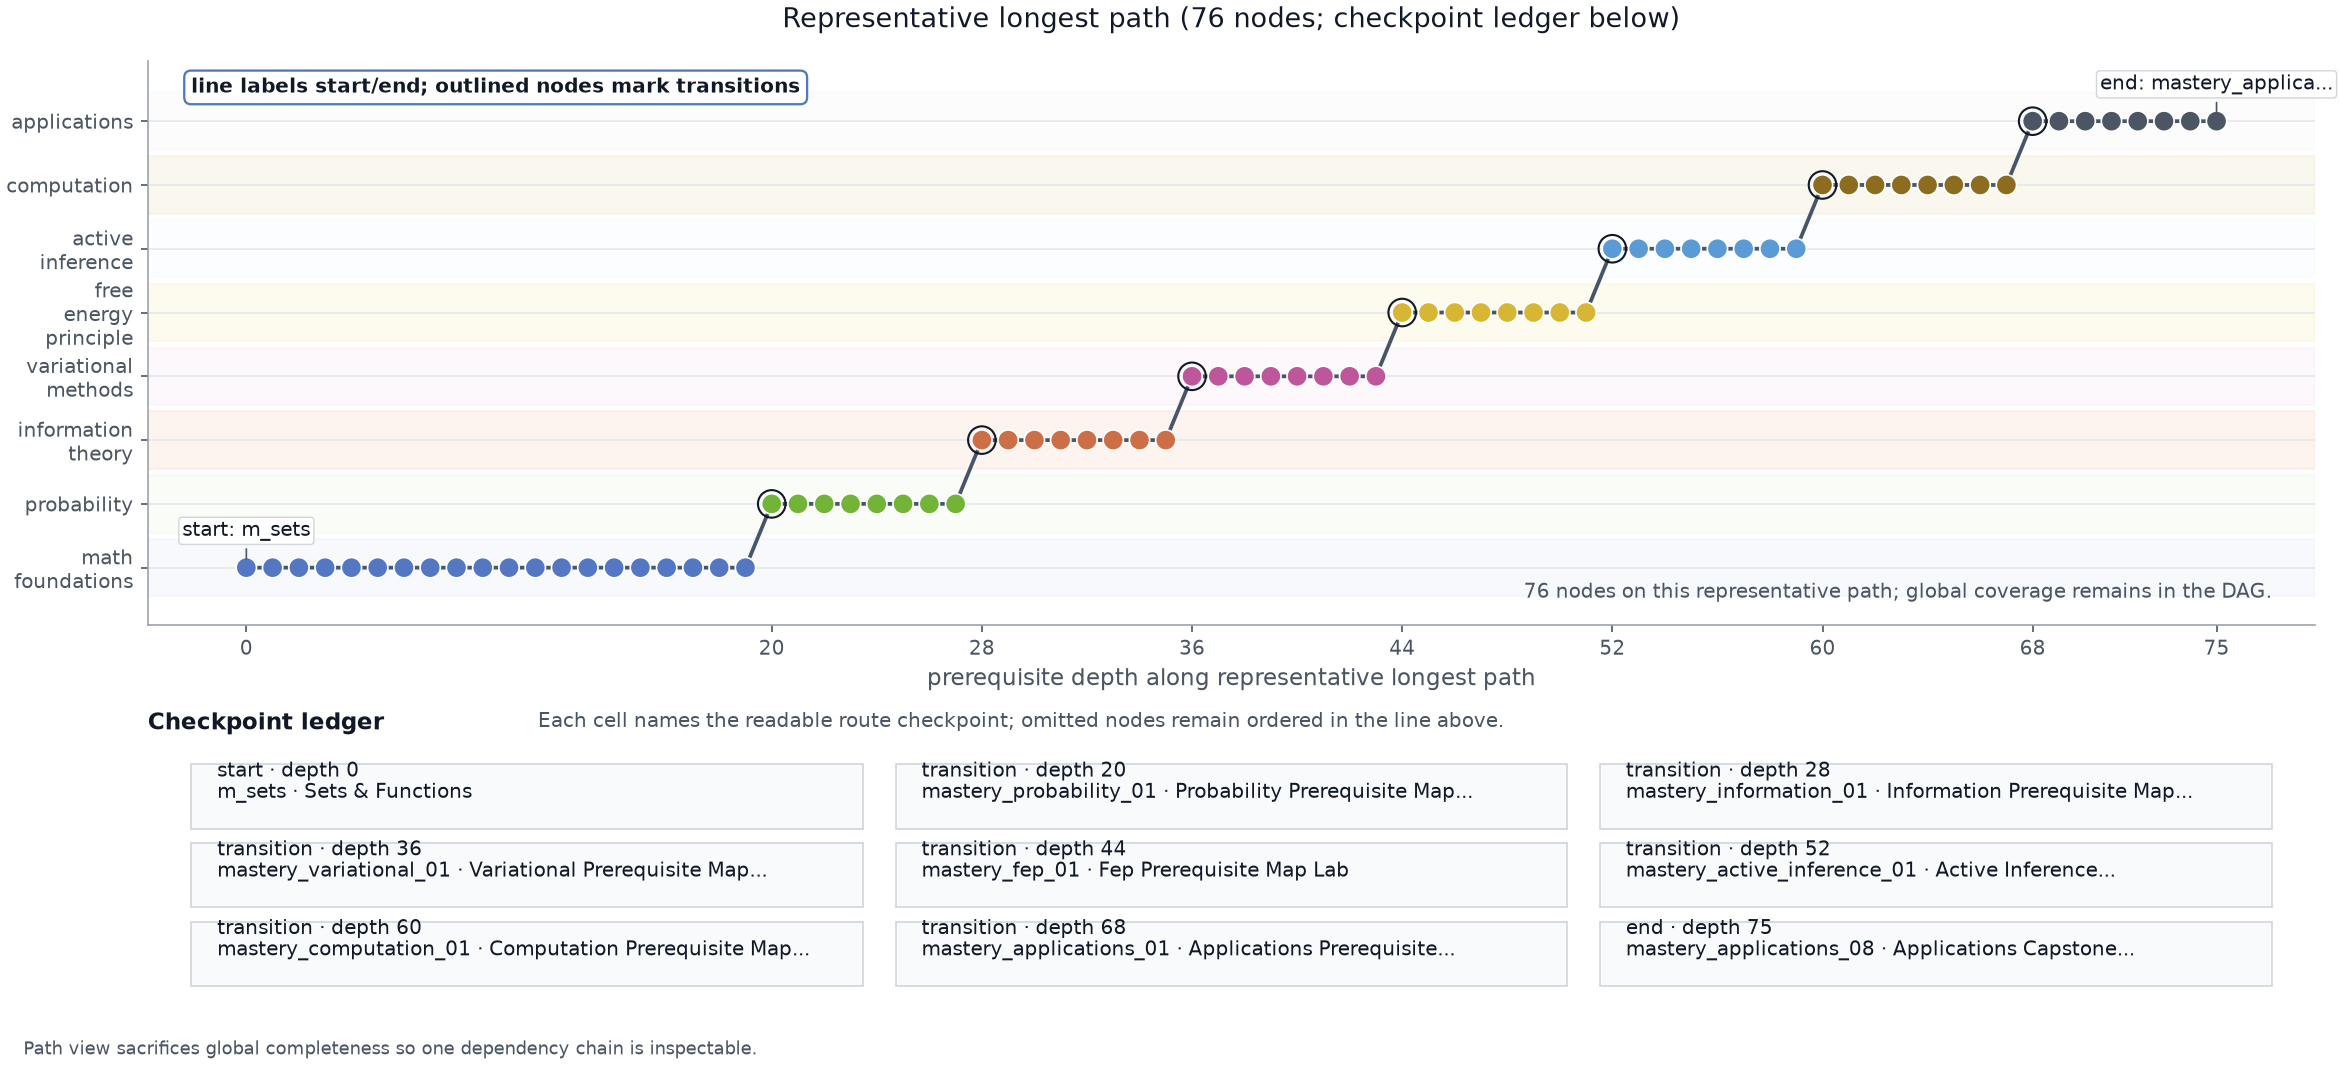
\includegraphics[width=1\linewidth,height=0.40\textheight,keepaspectratio,alt={Representative skill-neighborhood path generated from the longest-path diagnostic in the current graph. The line orders skills by prerequisite depth, stratum bands and vertical position encode pedagogical layer, and a checkpoint ledger names the start, every stratum transition, and the endpoint. This view deliberately trades global completeness for readability: it lets authors audit one concrete foundation-to-application pathway without relying on the dense full-DAG overview or tiny rotated labels.}]{../figures/skill_neighborhood_paths.png}
\caption{Representative skill-neighborhood path generated from the
longest-path diagnostic in the current graph. The line orders skills by
prerequisite depth, stratum bands and vertical position encode
pedagogical layer, and a checkpoint ledger names the start, every
stratum transition, and the endpoint. This view deliberately trades
global completeness for readability: it lets authors audit one concrete
foundation-to-application pathway without relying on the dense full-DAG
overview or tiny rotated labels.}\label{fig:skill_neighborhood_paths}
\end{figure}

\end{frame}

\begin{frame}[allowframebreaks]{Graph validity, prerequisite depth, and
assessment-quality gates}
fig.~\ref{fig:semantic_prerequisite_coverage} audits the
semantic-prerequisite gate, which checks that no skill is assessed on
one of the gate's tracked load-bearing concepts unless a skill defining
that concept sits in its transitive prerequisite closure. The gate reads
assessment text only, and it considers only definers at or before the
using skill's own stratum, so a forward reference to a later concept is
not counted as a missing prerequisite. For each concept the figure
reports how many skills reach the defining skill through their
prerequisite closure and how many are assessed on the concept, so an
inversion in which a learner met a concept before they could have
learned it would be visible rather than buried in the dense graph.

\end{frame}

\begin{frame}[allowframebreaks]{Graph validity, prerequisite depth, and
assessment-quality gates}
\begin{figure}
\centering
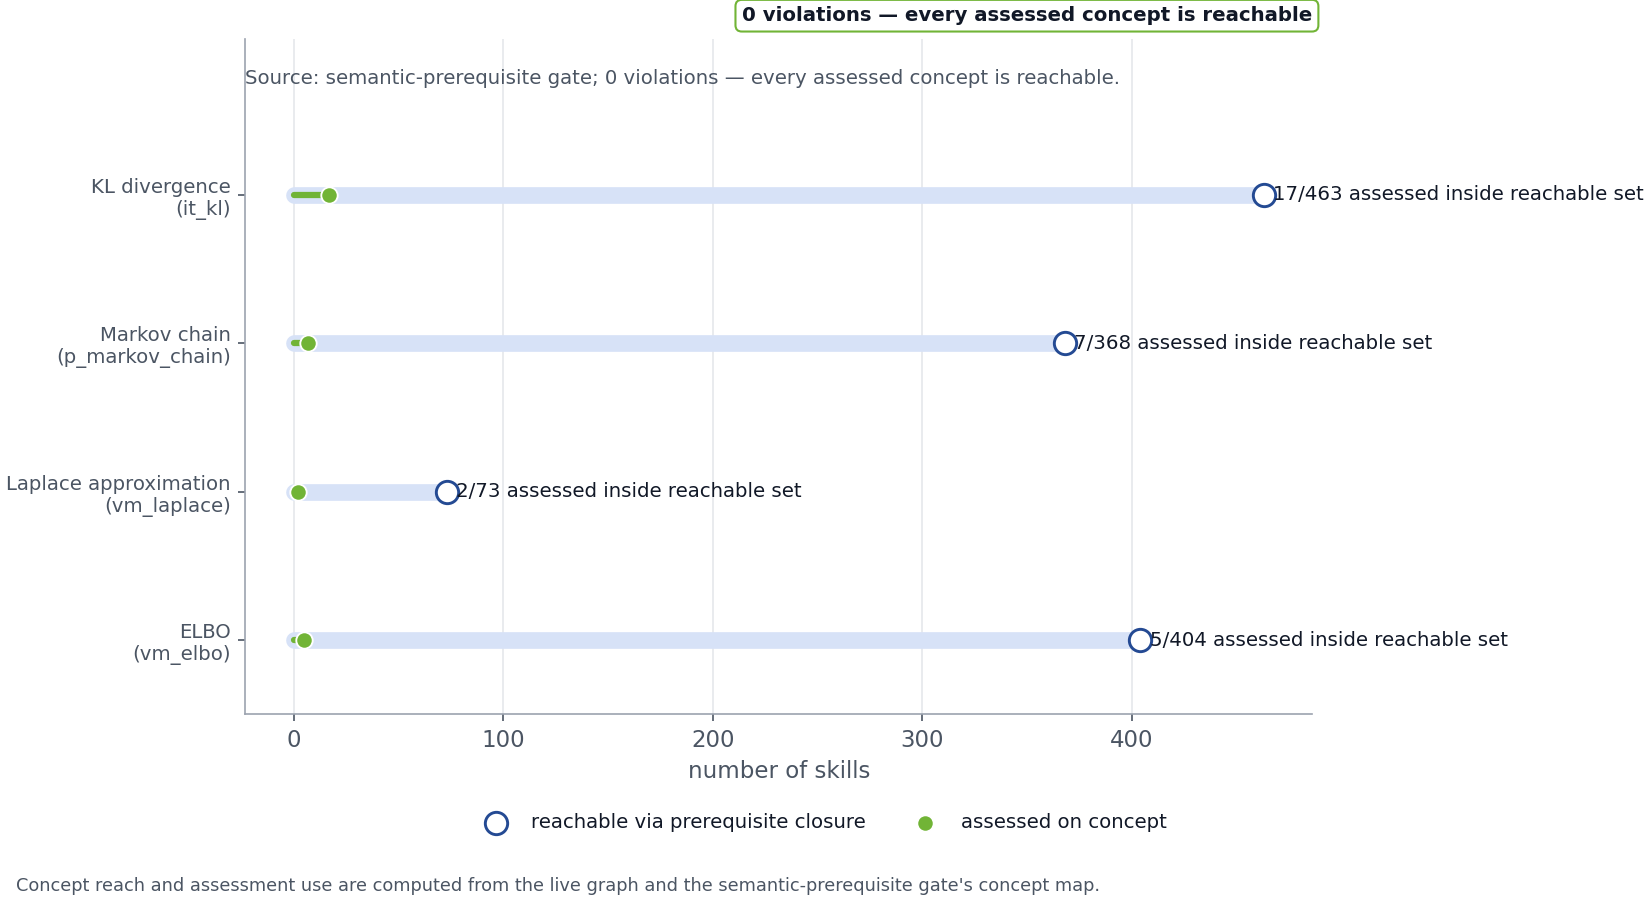
\includegraphics[width=0.92\linewidth,height=0.40\textheight,keepaspectratio,alt={Semantic-prerequisite coverage generated from the live graph and the quality gate's concept map. For each load-bearing concept the open marker and stem report skills whose prerequisite closure reaches the concept's defining skill, while the filled marker and direct label report the assessed subset inside that reachable set. The subtitle and badge report the gate verdict so a passing curriculum shows zero skills tested on a concept they could not yet have learned.}]{../figures/semantic_prerequisite_coverage.png}
\caption{Semantic-prerequisite coverage generated from the live graph
and the quality gate's concept map. For each load-bearing concept the
open marker and stem report skills whose prerequisite closure reaches
the concept's defining skill, while the filled marker and direct label
report the assessed subset inside that reachable set. The subtitle and
badge report the gate verdict so a passing curriculum shows zero skills
tested on a concept they could not yet have
learned.}\label{fig:semantic_prerequisite_coverage}
\end{figure}

\end{frame}

\begin{frame}[allowframebreaks]{Graph validity, prerequisite depth, and
assessment-quality gates}
The quiz surface is itself part of the curriculum result rather than a
decorative add-on. fig.~\ref{fig:assessment_depth} summarizes the
assessment-depth invariant by stratum. Every skill now carries the same
4-question floor, so completion is not certified by a single recognition
item or by a thin two-question check.

\end{frame}

\begin{frame}[allowframebreaks]{Graph validity, prerequisite depth, and
assessment-quality gates}
\begin{figure}
\centering
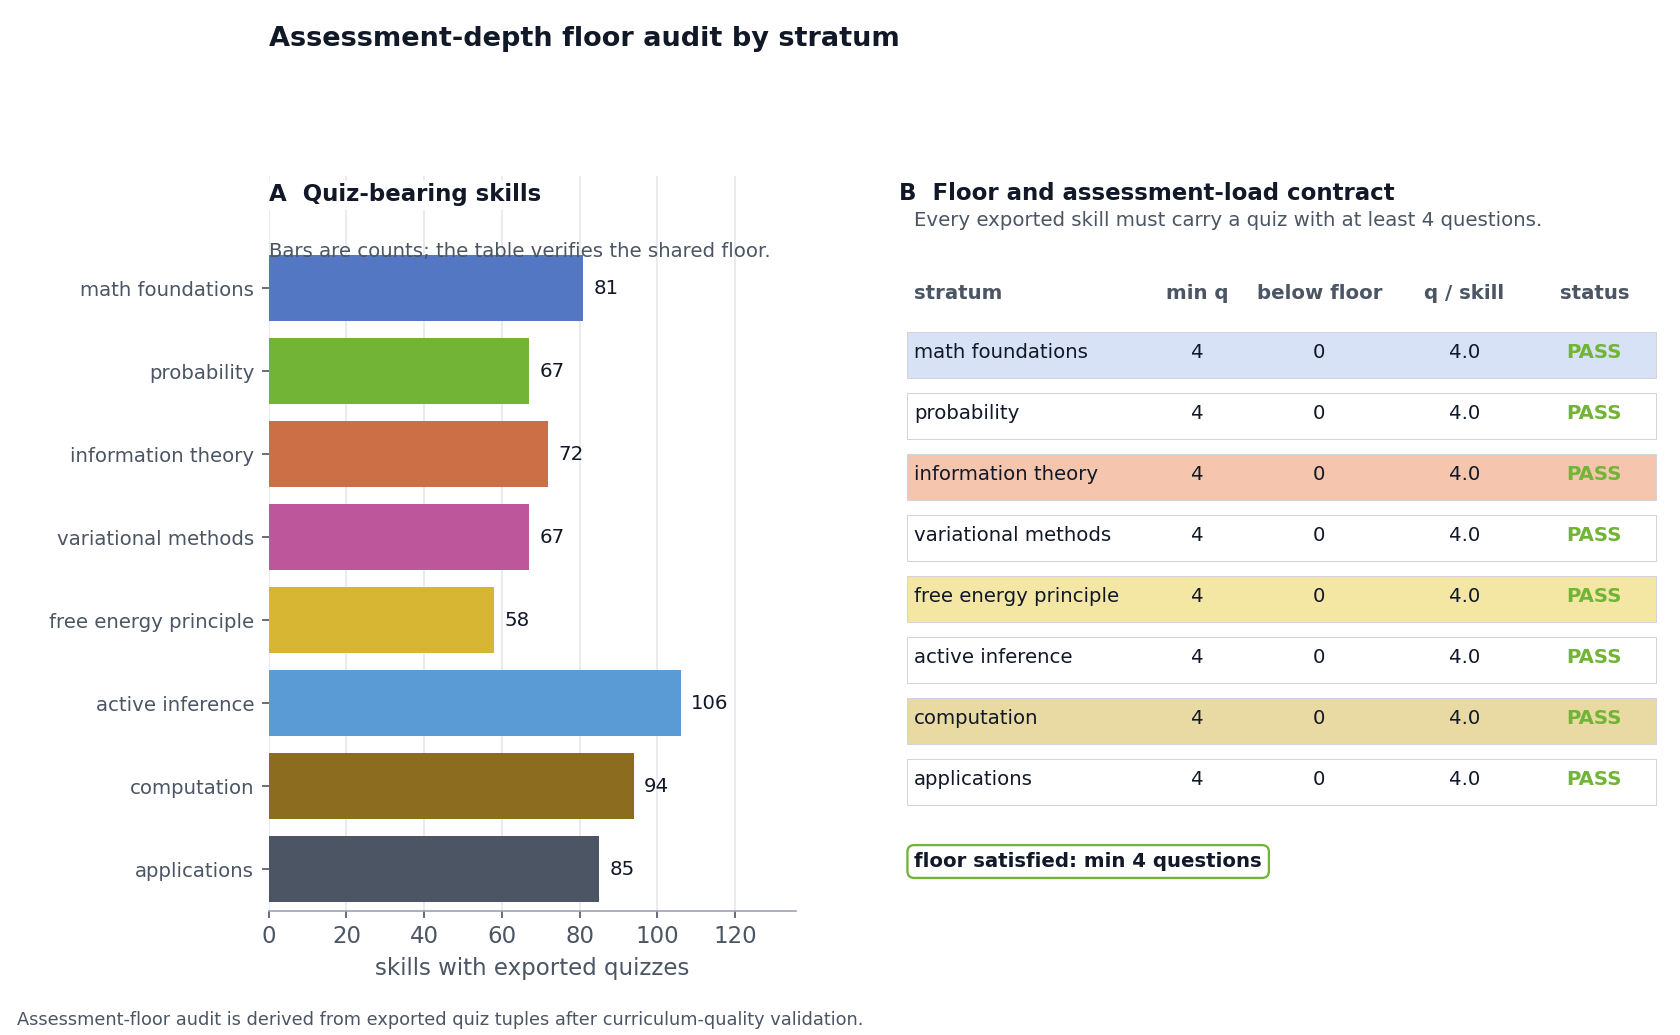
\includegraphics[width=0.9\linewidth,height=0.40\textheight,keepaspectratio,alt={Quiz assessment depth by stratum generated from the skill assessment tuples. The bar panel counts quiz-bearing skills per pedagogical stratum, and the accompanying audit table reports, per stratum, the minimum questions per skill, below-floor counts, questions per skill, and a PASS/REVIEW verdict against the configured 4-question failable floor. The intended check is not average quiz length but minimum learner friction: any below-floor mass would show that a skill can be completed without the configured 4-question floor.}]{../figures/assessment_depth_matrix.png}
\caption{Quiz assessment depth by stratum generated from the skill
assessment tuples. The bar panel counts quiz-bearing skills per
pedagogical stratum, and the accompanying audit table reports, per
stratum, the minimum questions per skill, below-floor counts, questions
per skill, and a PASS/REVIEW verdict against the configured 4-question
failable floor. The intended check is not average quiz length but
minimum learner friction: any below-floor mass would show that a skill
can be completed without the configured 4-question
floor.}\label{fig:assessment_depth}
\end{figure}

\end{frame}

\begin{frame}[allowframebreaks]{Graph validity, prerequisite depth, and
assessment-quality gates}
The latest expansion also needs a balance check.
fig.~\ref{fig:stratum_balance} summarizes skills, subjects, assessment
questions and incoming prerequisite edges by stratum. This makes a
different false-certification path visible: the graph can be larger
while still overloading one pedagogical layer or leaving another
underdeveloped.

\end{frame}

\begin{frame}[allowframebreaks]{Graph validity, prerequisite depth, and
assessment-quality gates}
\begin{figure}
\centering
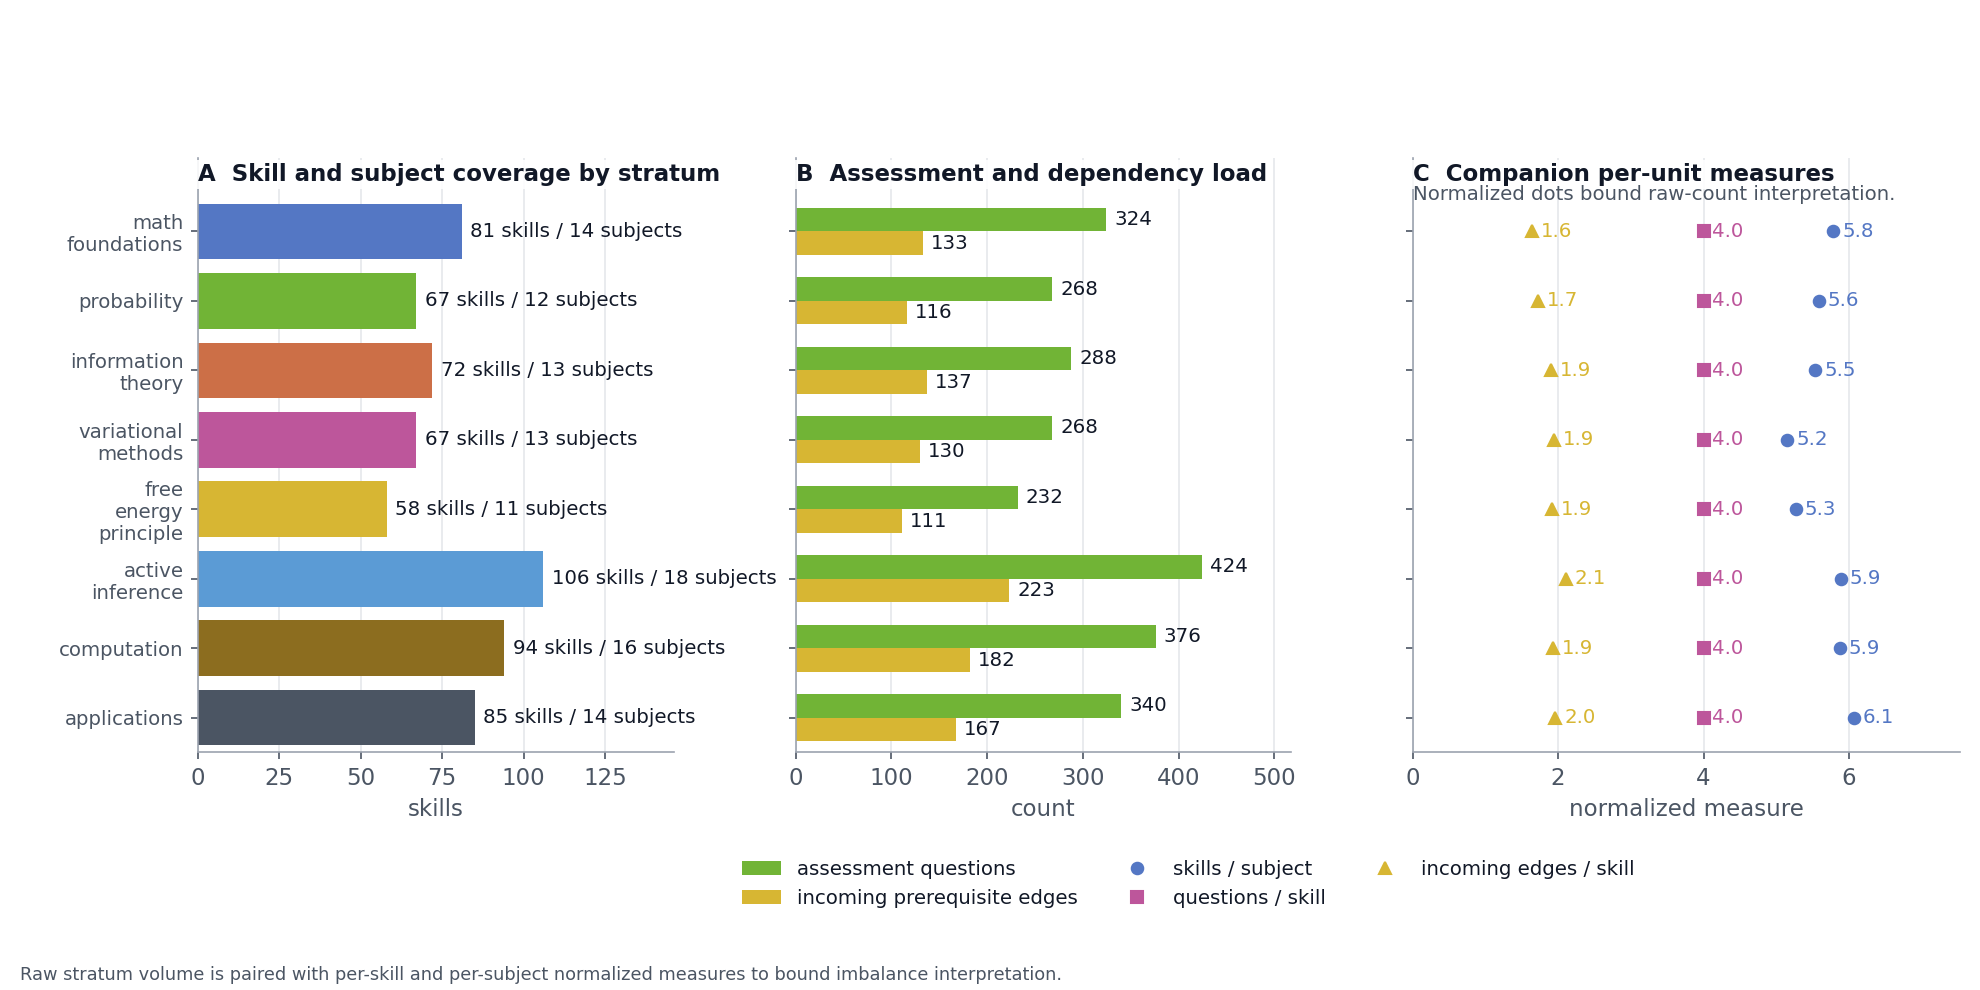
\includegraphics[width=1\linewidth,height=0.40\textheight,keepaspectratio,alt={Curriculum stratum-balance audit generated from current graph statistics after structural checks. Three panels report the same underlying build: the left panel shows skills and subjects per pedagogical stratum, the middle panel shows assessment-question volume and incoming prerequisite edges, and the right panel shows companion per-unit (per-skill and per-subject) normalized measures. Reading the panels together shows whether expansion is distributed across the learning path or whether one layer is absorbing disproportionate topic, quiz, or dependency load. The figure bounds the claim to catalog structure; it does not measure learner outcomes.}]{../figures/curriculum_stratum_balance.png}
\caption{Curriculum stratum-balance audit generated from current graph
statistics after structural checks. Three panels report the same
underlying build: the left panel shows skills and subjects per
pedagogical stratum, the middle panel shows assessment-question volume
and incoming prerequisite edges, and the right panel shows companion
per-unit (per-skill and per-subject) normalized measures. Reading the
panels together shows whether expansion is distributed across the
learning path or whether one layer is absorbing disproportionate topic,
quiz, or dependency load. The figure bounds the claim to catalog
structure; it does not measure learner
outcomes.}\label{fig:stratum_balance}
\end{figure}

\end{frame}

\begin{frame}[allowframebreaks]{Graph validity, prerequisite depth, and
assessment-quality gates}
Having established the graph surface, the next result is source support.
These audits ask whether the manuscript's scholarly claims are connected
to the roles its citations are supposed to play.
\end{frame}

\end{document}
